\documentclass[aspectratio=169]{beamer}
\usetheme{Madrid}
\usecolortheme{beaver}
\usepackage[utf8]{inputenc}
\usepackage[T1]{fontenc}
\usepackage{tikz}
\usepackage{amssymb}
\usepackage{graphicx}
\setbeamertemplate{navigation symbols}{}
\setbeamercolor{title}{fg=white,bg=cyan!60!black}
\setbeamercolor{frametitle}{fg=white,bg=cyan!50!black}
\setbeamercolor{block title}{bg=cyan!15,fg=black}
\setbeamercolor{block body}{bg=cyan!5,fg=black}

\title{G4 — My Blocks}
\subtitle{Lesson 1: spawnEnemy()}
\author{ByteForge --- Grade 7 --- Game Maker}
\date{}

\begin{document}

\begin{frame}
    \titlepage
\end{frame}

\begin{frame}{Functions — reusable named blocks}
    \Large
    A function is defined ONCE with parameters, then CALLED many times with different values — one definition, many different outcomes.

    \begin{center}
    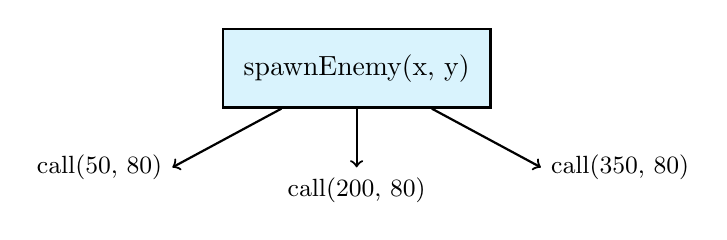
\begin{tikzpicture}[scale=0.9]

        \node[draw, thick, minimum width=3.4cm, minimum height=1cm, fill=cyan!15] (f) at (0,0) {spawnEnemy(x, y)};
        \draw[->, thick] (f) -- (-2.6,-1.4) node[left]{\small call(50, 80)};
        \draw[->, thick] (f) -- (0,-1.4) node[below]{\small call(200, 80)};
        \draw[->, thick] (f) -- (2.6,-1.4) node[right]{\small call(350, 80)};
    \end{tikzpicture}
    \end{center}
\end{frame}

\begin{frame}{Functions — reusable named blocks --- Worked Example}
    \Large
    Worked example: Minecraft's /function command (a real, named, reusable set of commands you can "call" from anywhere) is the exact same idea this chapter teaches — define once, invoke many times.
\end{frame}

\begin{frame}{Your Turn}
    \Large
    Open the student map, find \textbf{G4 — My Blocks}, and complete
    the \textbf{spawnEnemy()} challenge --- everything you just saw, they now do themselves.
\end{frame}

\end{document}
